% Options for packages loaded elsewhere
\PassOptionsToPackage{unicode}{hyperref}
\PassOptionsToPackage{hyphens}{url}
\documentclass[
]{article}
\usepackage{xcolor}
\usepackage[margin=1in]{geometry}
\usepackage{amsmath,amssymb}
\usepackage[inkscapeversion=1]{svg}
\setcounter{secnumdepth}{-\maxdimen} % remove section numbering
\usepackage{iftex}
\ifPDFTeX
  \usepackage[T1]{fontenc}
  \usepackage[utf8]{inputenc}
  \usepackage{textcomp} % provide euro and other symbols
\else % if luatex or xetex
  \usepackage{unicode-math} % this also loads fontspec
  \defaultfontfeatures{Scale=MatchLowercase}
  \defaultfontfeatures[\rmfamily]{Ligatures=TeX,Scale=1}
\fi
\usepackage{lmodern}
\ifPDFTeX\else
  % xetex/luatex font selection
\fi
% Use upquote if available, for straight quotes in verbatim environments
\IfFileExists{upquote.sty}{\usepackage{upquote}}{}
\IfFileExists{microtype.sty}{% use microtype if available
  \usepackage[]{microtype}
  \UseMicrotypeSet[protrusion]{basicmath} % disable protrusion for tt fonts
}{}
\makeatletter
\@ifundefined{KOMAClassName}{% if non-KOMA class
  \IfFileExists{parskip.sty}{%
    \usepackage{parskip}
  }{% else
    \setlength{\parindent}{0pt}
    \setlength{\parskip}{6pt plus 2pt minus 1pt}}
}{% if KOMA class
  \KOMAoptions{parskip=half}}
\makeatother
\usepackage{color}
\usepackage{fancyvrb}
\newcommand{\VerbBar}{|}
\newcommand{\VERB}{\Verb[commandchars=\\\{\}]}
\DefineVerbatimEnvironment{Highlighting}{Verbatim}{commandchars=\\\{\}}
% Add ',fontsize=\small' for more characters per line
\newenvironment{Shaded}{}{}
\newcommand{\AlertTok}[1]{\textcolor[rgb]{1.00,0.00,0.00}{\textbf{#1}}}
\newcommand{\AnnotationTok}[1]{\textcolor[rgb]{0.38,0.63,0.69}{\textbf{\textit{#1}}}}
\newcommand{\AttributeTok}[1]{\textcolor[rgb]{0.49,0.56,0.16}{#1}}
\newcommand{\BaseNTok}[1]{\textcolor[rgb]{0.25,0.63,0.44}{#1}}
\newcommand{\BuiltInTok}[1]{\textcolor[rgb]{0.00,0.50,0.00}{#1}}
\newcommand{\CharTok}[1]{\textcolor[rgb]{0.25,0.44,0.63}{#1}}
\newcommand{\CommentTok}[1]{\textcolor[rgb]{0.38,0.63,0.69}{\textit{#1}}}
\newcommand{\CommentVarTok}[1]{\textcolor[rgb]{0.38,0.63,0.69}{\textbf{\textit{#1}}}}
\newcommand{\ConstantTok}[1]{\textcolor[rgb]{0.53,0.00,0.00}{#1}}
\newcommand{\ControlFlowTok}[1]{\textcolor[rgb]{0.00,0.44,0.13}{\textbf{#1}}}
\newcommand{\DataTypeTok}[1]{\textcolor[rgb]{0.56,0.13,0.00}{#1}}
\newcommand{\DecValTok}[1]{\textcolor[rgb]{0.25,0.63,0.44}{#1}}
\newcommand{\DocumentationTok}[1]{\textcolor[rgb]{0.73,0.13,0.13}{\textit{#1}}}
\newcommand{\ErrorTok}[1]{\textcolor[rgb]{1.00,0.00,0.00}{\textbf{#1}}}
\newcommand{\ExtensionTok}[1]{#1}
\newcommand{\FloatTok}[1]{\textcolor[rgb]{0.25,0.63,0.44}{#1}}
\newcommand{\FunctionTok}[1]{\textcolor[rgb]{0.02,0.16,0.49}{#1}}
\newcommand{\ImportTok}[1]{\textcolor[rgb]{0.00,0.50,0.00}{\textbf{#1}}}
\newcommand{\InformationTok}[1]{\textcolor[rgb]{0.38,0.63,0.69}{\textbf{\textit{#1}}}}
\newcommand{\KeywordTok}[1]{\textcolor[rgb]{0.00,0.44,0.13}{\textbf{#1}}}
\newcommand{\NormalTok}[1]{#1}
\newcommand{\OperatorTok}[1]{\textcolor[rgb]{0.40,0.40,0.40}{#1}}
\newcommand{\OtherTok}[1]{\textcolor[rgb]{0.00,0.44,0.13}{#1}}
\newcommand{\PreprocessorTok}[1]{\textcolor[rgb]{0.74,0.48,0.00}{#1}}
\newcommand{\RegionMarkerTok}[1]{#1}
\newcommand{\SpecialCharTok}[1]{\textcolor[rgb]{0.25,0.44,0.63}{#1}}
\newcommand{\SpecialStringTok}[1]{\textcolor[rgb]{0.73,0.40,0.53}{#1}}
\newcommand{\StringTok}[1]{\textcolor[rgb]{0.25,0.44,0.63}{#1}}
\newcommand{\VariableTok}[1]{\textcolor[rgb]{0.10,0.09,0.49}{#1}}
\newcommand{\VerbatimStringTok}[1]{\textcolor[rgb]{0.25,0.44,0.63}{#1}}
\newcommand{\WarningTok}[1]{\textcolor[rgb]{0.38,0.63,0.69}{\textbf{\textit{#1}}}}
\usepackage{longtable,booktabs,array}
\usepackage{calc} % for calculating minipage widths
% Correct order of tables after \paragraph or \subparagraph
\usepackage{etoolbox}
\makeatletter
\patchcmd\longtable{\par}{\if@noskipsec\mbox{}\fi\par}{}{}
\makeatother
% Allow footnotes in longtable head/foot
\IfFileExists{footnotehyper.sty}{\usepackage{footnotehyper}}{\usepackage{footnote}}
\makesavenoteenv{longtable}
\usepackage{graphicx}
\makeatletter
\newsavebox\pandoc@box
\newcommand*\pandocbounded[1]{% scales image to fit in text height/width
  \sbox\pandoc@box{#1}%
  \Gscale@div\@tempa{\textheight}{\dimexpr\ht\pandoc@box+\dp\pandoc@box\relax}%
  \Gscale@div\@tempb{\linewidth}{\wd\pandoc@box}%
  \ifdim\@tempb\p@<\@tempa\p@\let\@tempa\@tempb\fi% select the smaller of both
  \ifdim\@tempa\p@<\p@\scalebox{\@tempa}{\usebox\pandoc@box}%
  \else\usebox{\pandoc@box}%
  \fi%
}
% Set default figure placement to htbp
\def\fps@figure{htbp}
\makeatother
\setlength{\emergencystretch}{3em} % prevent overfull lines
\providecommand{\tightlist}{%
  \setlength{\itemsep}{0pt}\setlength{\parskip}{0pt}}
\usepackage{bookmark}
\IfFileExists{xurl.sty}{\usepackage{xurl}}{} % add URL line breaks if available
\urlstyle{same}
\hypersetup{
  hidelinks,
  pdfcreator={LaTeX via pandoc}}

\author{}
\date{}

\begin{document}


\begin{center}
  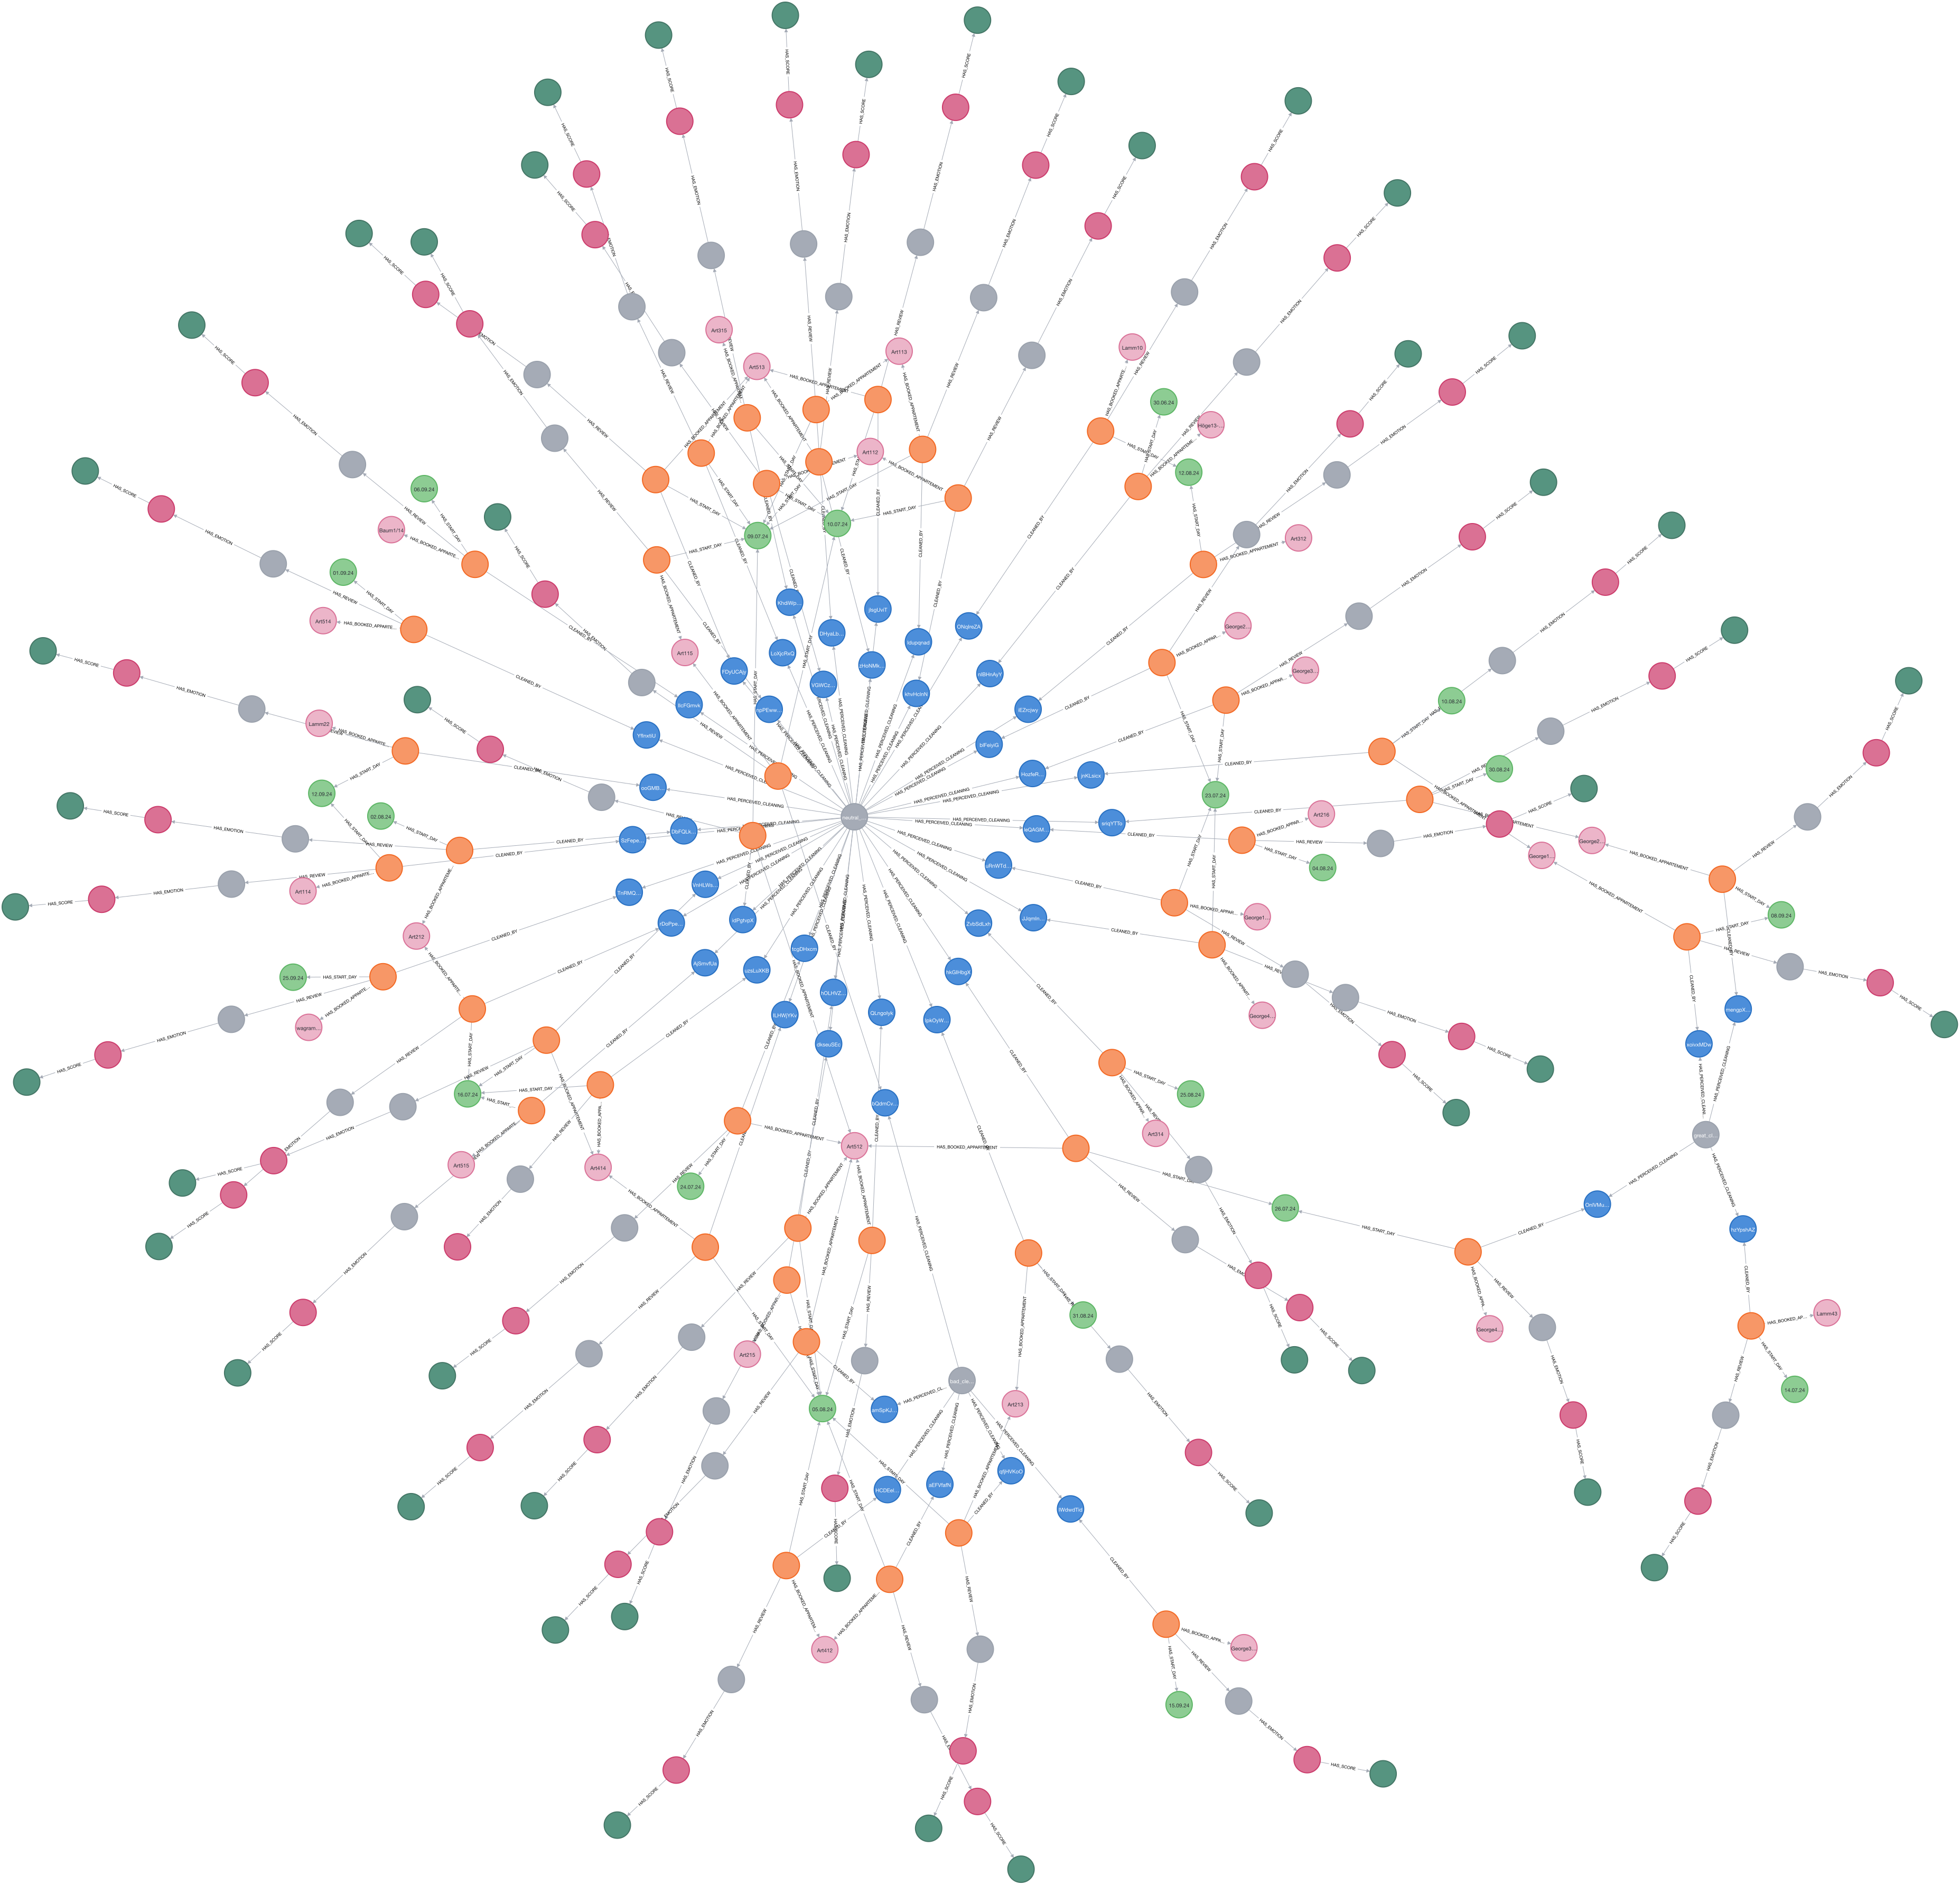
\includegraphics[width=0.7\textwidth]{drawings/graph_fully_con.png}
\end{center}


\section{1. Introduction}\label{introduction}

\subsection{1.1 Scenario}\label{scenario}

Short-Term Renting business (STR) is hard, but without the right
monitoring tools for customer satisfaction, it is even harder (then it
has to be). This Project utilizes modern Knowledge-Graph-based
Approaches to assist hotels and STR-businesses in \textbf{identifying
key issues} regarding their cleaning services and customer
satisfactions. In particular, it aims to identify whether certain
apartments or cleaning staff form clusters or sources of exceptionally
good or bad customer experiences.

\subsubsection{1.1.1 Proposed Analytics and
Solutions}\label{proposed-analytics-and-solutions}

For this reason, this project aims to provide a presentation layer (via
a \texttt{streamlit} application) that displays the following
information to the user: - A list of cleaning personal that is linked to
the best/worst customer experiences. - A list of apartments that are
linked to the best/worst customer experiences. - An analysis to identify
if certain cleaning people or appartements became a central node in a
node of bad customer experiences or form a cluster utilizing utilizing
\emph{Deep Modularity Networks}. - A list of cleaners that are assumed
to have a high record of bad cleaning quality, which is determined
through the use of a Graph Embedding-Technique (\emph{TransE}) that
learns whether a review indicates a bad cleaning quality.

Eventually, this insight could then be used to infer insights for
improvements in cleaning protocols, appartements and eventually customer
satisfaction.

\subsection{1.2 Background}\label{background}

In the hotel/STR business, a common SaaS Stack is the combination of
\href{https://www.krossbooking.com/en}{Kross Booking} that provides PMS
+ Channel Manager + Booking Engine in one solution, in combination with
\href{https://www.timetac.com/en/}{TimeTac} that allows for smart time
tracking of all internal (cleaning) processes. While the above is great
for managing daily operations, the amount of data insight that can be
extracted out of the box is pretty limited and Hence, business owners of
certain scales that use the SaaS stack described above are left with
high amounts of manual analytical effort with still limited insights.\\
Therefore, this project tries to reduce the amount of manual effort
needed, as well as to increase the quality of insight possible.

\section{2. Data Source}\label{data-source}

In order to achieve the previously defined objectives, the following
data has been used to construct a Knowledgegraph (based on an ontology,
depicted later on in the architecture section) from two APIs:

\subsection{2.1 Raw Data}\label{raw-data}

\subsubsection{2.1.1 Kross Booking}\label{kross-booking}

As mentioned before, this is a plattform that works as booking engine
for the management of hotels/appartements. In this context, it is used
to oversee (and store) all bookings and related activities across all
properties. The stored data about the bookings can be fetched via a
REST-API following the OpenAPI Standard. \#\#\# 2.1.2 TimeTac A
plattform that allows to track process times of (cleaning) people. In
this instance, it is utilized to track and access data regarding who
cleaned each apartment, along with the timing and duration of the
cleaning. The stored data about cleaning durations can be fetched via a
REST-API following the OpenAPI Standard

\subsection{2.2 Additionally derived
Data}\label{additionally-derived-data}

In addition, the collected reviews (via \emph{Kross Booking}) are
automatically translated and pre-evaluated with a sentiment model.\\
\#\#\# 2.2.1 Translation As the customers of the appartements can (and
have been) writing reviews in more than 150 different languages, I had
to start out by translating them to a single language. For this purpose,
I used the \texttt{src/review\_process\_utils/review\_translor.py}
script that utilizes the \texttt{googleTrans} package to translate all
reviews (if possible) to english.

\subsubsection{2.2.2 Sentiment Analysis}\label{sentiment-analysis}

In addition, for effective review analysis, a sentiment analysis
utilizing
\href{https://huggingface.co/j-hartmann/emotion-english-distilroberta-base}{DistilRoBERTa}
has been implemented to categorize the reviews along
\href{https://www.paulekman.com/wp-content/uploads/2013/07/Basic-Emotions.pdf}{Paul
Ekman's 6 basic dimensions} + one neural dimension in case no particular
emotion has been detected. The corresponding script can be found in
\texttt{src/Review\_Handler.py}

\subsubsection{2.2.3 Results}\label{results}

The two additional operations, the translation and sentiment analysis
then yielded the following additional review data per Booking\_ID for
the knowledge graph:

\begin{longtable}[]{@{}ll@{}}
\toprule\noalign{}
Column Name & Data Type \\
\midrule\noalign{}
\endhead
\bottomrule\noalign{}
\endlastfoot
Booking\_ID (PK) & INT \\
Translated\_Review\_Text & TEXT \\
Primary\_Emotion & TEXT \\
Sentiment\_Score & FLOAT \\
Cleaning\_Quality & INT \\
\end{longtable}

To simplify data management, this information is also stored in AWS RDS.
Of course arguments for storing this data in a NoSQL Table like MongoDB
or AWS Dynamo DB can be made, but due to the limited scope of this
project I have decided to keep the overhead low and not setup another
DB.

\subsection{2.3 Data for the
Knowledge-Graph-Generation}\label{data-for-the-knowledge-graph-generation}

Finally, the resulting data has been stored in the following ABT
\texttt{ABT\_BASE\_TABLE\_KG\_GENERATION} that will be used for building
the Knowledge Graph:

\begin{longtable}[]{@{}lll@{}}
\toprule\noalign{}
Column Name & Data Type & Source \\
\midrule\noalign{}
\endhead
\bottomrule\noalign{}
\endlastfoot
Booking\_ID (PK) & INT & KROSS \\
Start\_date\_of\_stay & TIME STAMP & KROSS \\
Appartement & STRING & KROSS \\
Cleaner & STRING & TIMETAC \\
Translated\_Review\_Text & TEXT & KROSS \\
Primary\_Emotion & TEXT & ML Model \\
Sentiment\_Score & FLOAT & ML Model \\
Quality\_Indication & INT & Manual/TransE \\
\end{longtable}

\textbf{Side Notes:} - For this demonstration purpose, the production
data has been used and been anonymized using
\texttt{src/data\_anonimizer.py} and stored in
\texttt{data/demo\_data.csv} - Given my limited local computational
resources, I have opted to work with a small sample of the original
data. However, the project is designed to be scalable, allowing for the
entire dataset to be efficiently processed by deploying it to AWS with
additional computational resources.

\section{3. KGMS and KG Construction}\label{kgms-and-kg-construction}

As mentioned before, the application utilizes data that has been fetched
from \emph{KROSS Booking} and \emph{TimeTac} via their internal APIs is
currently stored in a AWS RDS in multiple tables using the architecture
displayed below:


\begin{center}
  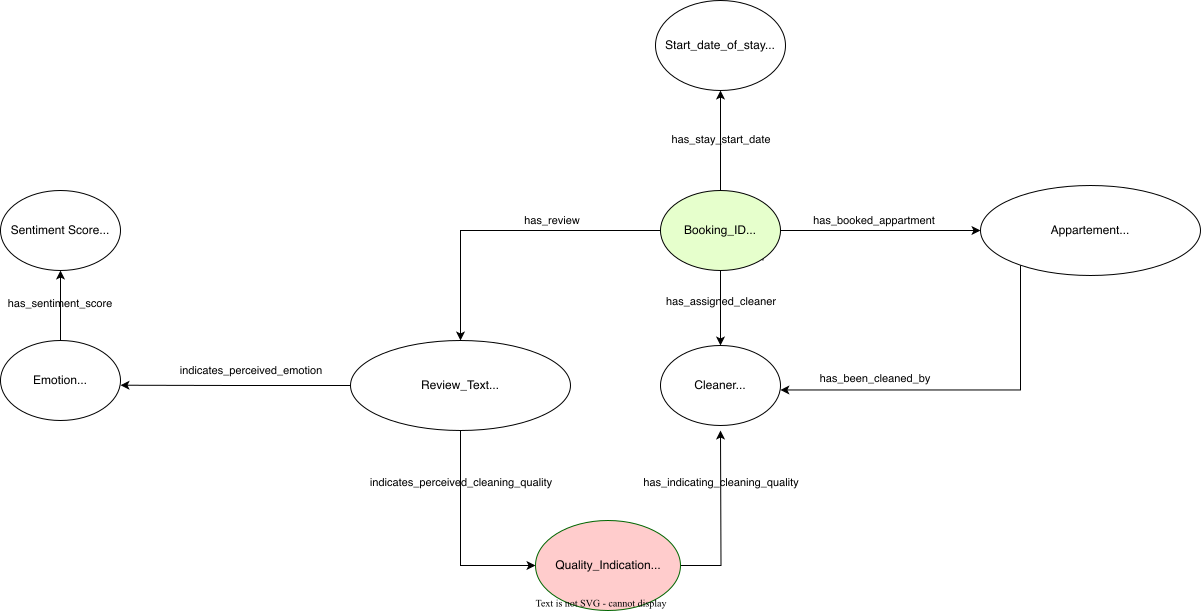
\includegraphics[width=0.7\textwidth]{drawings/Application_Architecture.png}
\end{center}
\pagebreak

In the beginning the data is being fetched from the two API's utilizing
a python script that runs in a \emph{AWS Lamda Container} that is being
executed once per day (at midnight). Once the data has been fetched
successfully, is then stored in extraction tables in a \emph{PostgreSQL}
DB stored in an \emph{AWS RDS Instance} (serving as central source of
truth) and then automatically (via \emph{AWS Lamda} again) processed
into the aforementioned ABT.

In the meantime, an adapter (also running in a different \emph{AWS Lamda
Container}), is daily fetching new review data from the ABT, sends the
reviews to a sentiment model (\texttt{emotion\_detector.py}) that
returns the top sentiment scores for each review.

After that, the data gets transformed into a graph-structure and then
added to an on-premise \emph{Neo4J} Database (dockerized) via the
following python script \texttt{src/KG\_Building\_Handler.py}. This
script iterates over every row in the ABT, transforms it based on the
Ontology below and adds it to Neo4j. In case a certain Node already
exists (for example, an appartement has already been booked before), the
script uses Cypher to determine this and instead of creating a new node
of this kind, the already existing ndoe will be used.

Through the process outlined above, the Knowledge Graph (KG) is updated
daily with the latest available data, allowing it to continuously
evolve. The resulting KG comprises a collection of nodes and edges. Each
row in the ABT corresponds to one such instance displayed below.


\pandocbounded{\includesvg[keepaspectratio]{drawings/KG_Architecture.svg}}


\textbf{Side Notes:} - In the initial creation phase, edges leading to
the \emph{Quality Indication} are available only for a specific subgroup
(the training set). These edges are intended to be learned using
\emph{TransE}.

\subsection{3.1 Technologies used:}\label{technologies-used}

Starting out, EC2 (running \emph{Python} and \emph{PostgreSQL}) and
\(\lamda\) have been chosen for the data engineering side, including job
scheduling and classic RDBS (using PostgreSQL as Single Source of
Truth). The decision to adopt this technology suite was mainly
influenced by it's general purpose, time proven quality, high
scalability and wide array of utilities. In addition, it provides a
strong architectural backbone for all kind of ML-Application, being it
classic, or graph based machine learning, allowing them to flourish in
harmony and synergy.

Furthermore \emph{Neo4j} was then chose as a graph database for storing
the built Knowledge Graph(s), while other database have been
investigated, some being: - Amazons's own solution - Neptune -
Microsoft's Azure Cosmos DB - Dgraph - ArangoDB - OrientDB - \ldots.

While each DB provided individual advantages and disadvantages, Neo4j
was convincing for this project, mainly due to it's great support for
graph data structure, Cypher's amazing syntax, the efficient querying
and the docker support, leading to great flexibility, solid performance,
and eas of use that was really appealing. The opportunity to add Neo4j
in a docker container to the existing technical infrastructure in AWS
(leveraging EC2) underlines the flexibility and scalability of this
technology.

In addition and out of curiosity (in Vadalog/Datalog), a \textbf{cozoDB}
has also been setup (can be found in \texttt{DataLogMe}) and tested. Due
to time constraints for further experiments, I nonetheless stuck to
Neo4j and Cypher.

\section{4 Analytics / Methods}\label{analytics-methods}

\subsection{4.1 Knowledge Graph
Embeddings}\label{knowledge-graph-embeddings}

\subsubsection{4.1.1 Introduction}\label{introduction-1}

One very important factor for customer satisfaction in this industry is
the quality of the appartement cleanings. With increasing numbers of
properties under management, assessing this quality can become a very
time-consuming and inefficient process. So the idea here is to offer the
business owners a application that helps to assess the quality of the
appartement cleanings. As this is a very specific use case, a general
(not fine-tuned and industry specific) model like BERT is assumed to be
only of limited help. Therefore, a very small train-dataset (due to the
time constraints) consisting of manually labels that indicate whether a
review is concerned with cleaning issues, has been created and used to
learn the \emph{indicates\_perceived\_cleaning\_quality} relationship
from the original ontology with the help of
\href{https://proceedings.neurips.cc/paper_files/paper/2013/file/1cecc7a77928ca8133fa24680a88d2f9-Paper.pdf}{TransE}
were the logic for the relationship connection should be the following:

\[
\text{Quality Indication(Review)} = 
\begin{cases}
\text{great cleaning quality}, & \text{If good cleaning explicitly mentioned }  \\
\text{neutral cleaning quality}, & \text{If no problems mentioned in the review }  \\ 
\text{bad cleaning quality}, & \text{Else }
\end{cases}
\]

Hence, the goal is to solve the following:

\begin{verbatim}
<img src="drawings/TransE_Goal.svg" alt="TransE Learning" style="width: 70%;">
\end{verbatim}

\subsubsection{4.1.2 Used Model(s)}\label{used-models}

To address this problem, I chose to use Knowledge Graph (KG) Embeddings.
Although I've tested only one algorithm, TransE, the code is designed
with the GoF's Strategy Pattern in mind. This approach allows for the
quick implementation of additional embedding algorithms available in the
\emph{PyKEEN} library, such as \emph{TransF}, \emph{PairRE},
\emph{QuatE}, and many others.

For now \emph{TransE} has been selected as suitable model and
trained/learned the following way:

\begin{verbatim}
<img src="drawings/img.png" alt="TransE Learning" style="width: 90%;">
\end{verbatim}

\begin{verbatim}
<img src="drawings/TransE_training.svg" alt="TransE Learning" style="width: 90%;">
\end{verbatim}

The implementation can be found in \texttt{src/Embeddings\_Handler.py}.

\subsubsection{4.1.3 Embeddings Results}\label{embeddings-results}

On the very small test-set the Model yielded the following proposed
connections. Although the small training set does not yield highly
sophisticated results, the framework developed here provides a scalable
solution that can be easily adapted for larger training and test sets,
as well as for making predictions.

\begin{longtable}[]{@{}
  >{\raggedright\arraybackslash}p{(\linewidth - 6\tabcolsep) * \real{0.6524}}
  >{\raggedright\arraybackslash}p{(\linewidth - 6\tabcolsep) * \real{0.1810}}
  >{\raggedright\arraybackslash}p{(\linewidth - 6\tabcolsep) * \real{0.1143}}
  >{\raggedright\arraybackslash}p{(\linewidth - 6\tabcolsep) * \real{0.0524}}@{}}
\toprule\noalign{}
\begin{minipage}[b]{\linewidth}\raggedright
Review\_Text
\end{minipage} & \begin{minipage}[b]{\linewidth}\raggedright
Edge
\end{minipage} & \begin{minipage}[b]{\linewidth}\raggedright
Quality\_Indication
\end{minipage} & \begin{minipage}[b]{\linewidth}\raggedright
score
\end{minipage} \\
\midrule\noalign{}
\endhead
\bottomrule\noalign{}
\endlastfoot
Everything was perfect! & indicates\_perceived\_cleaning\_quality &
bad\_cleaning\_quality & -0.608245 \\
Good for the price & indicates\_perceived\_cleaning\_quality &
bad\_cleaning\_quality & -0.475592 \\
Great stay & indicates\_perceived\_cleaning\_quality &
bad\_cleaning\_quality & -0.642992 \\
Great stay, thank you. & indicates\_perceived\_cleaning\_quality &
bad\_cleaning\_quality & -0.475699 \\
Great value. We slept 4 adults in two double beds, with a clean bathroom
and kitchen. & indicates\_perceived\_cleaning\_quality &
bad\_cleaning\_quality & -0.701354 \\
It was a great base for my travels, thank you! &
indicates\_perceived\_cleaning\_quality & bad\_cleaning\_quality &
-0.514512 \\
Nice and comfortable place. & indicates\_perceived\_cleaning\_quality &
bad\_cleaning\_quality & -0.594642 \\
Nice place to stay. Good value for money. &
indicates\_perceived\_cleaning\_quality & bad\_cleaning\_quality &
-0.520994 \\
Nice quiet hotel. Fastlane station to city center approx. 10 min away.
The room was clean but there were some bags of the guests before &
indicates\_perceived\_cleaning\_quality & great\_cleaning\_quality &
-0.988858 \\
Our stay was just amazing. The best location and a clean room. &
indicates\_perceived\_cleaning\_quality & bad\_cleaning\_quality &
-0.762633 \\
\end{longtable}

\subsection{4.2 GNNs and the KG}\label{gnns-and-the-kg}

\subsubsection{4.2.1 Introduction}\label{introduction-2}

The initial analysis focuses on high-density regions and grouping.
Specifically, I aim to determine if the entire graph can be clustered
into meaningful clusters. For this task, I based my approach on the
paper by
\href{https://www.jmlr.org/papers/volume24/20-998/20-998.pdf}{Tsitsulin
et.al. (2023)} In this paper, the authors have compared the following
different methods, including their basic properties and introduced their
own Methode \emph{Deep Modularity Networks} (\textbf{DMoN}).

\begin{longtable}[]{@{}
  >{\raggedright\arraybackslash}p{(\linewidth - 14\tabcolsep) * \real{0.1163}}
  >{\raggedright\arraybackslash}p{(\linewidth - 14\tabcolsep) * \real{0.1395}}
  >{\raggedright\arraybackslash}p{(\linewidth - 14\tabcolsep) * \real{0.0930}}
  >{\raggedright\arraybackslash}p{(\linewidth - 14\tabcolsep) * \real{0.1628}}
  >{\raggedright\arraybackslash}p{(\linewidth - 14\tabcolsep) * \real{0.0930}}
  >{\raggedright\arraybackslash}p{(\linewidth - 14\tabcolsep) * \real{0.1628}}
  >{\raggedright\arraybackslash}p{(\linewidth - 14\tabcolsep) * \real{0.0930}}
  >{\raggedright\arraybackslash}p{(\linewidth - 14\tabcolsep) * \real{0.1395}}@{}}
\toprule\noalign{}
\begin{minipage}[b]{\linewidth}\raggedright
Method
\end{minipage} & \begin{minipage}[b]{\linewidth}\raggedright
End-to-end
\end{minipage} & \begin{minipage}[b]{\linewidth}\raggedright
Unsup.
\end{minipage} & \begin{minipage}[b]{\linewidth}\raggedright
Node pooling
\end{minipage} & \begin{minipage}[b]{\linewidth}\raggedright
Sparse
\end{minipage} & \begin{minipage}[b]{\linewidth}\raggedright
Soft assign.
\end{minipage} & \begin{minipage}[b]{\linewidth}\raggedright
Stable
\end{minipage} & \begin{minipage}[b]{\linewidth}\raggedright
Complexity
\end{minipage} \\
\midrule\noalign{}
\endhead
\bottomrule\noalign{}
\endlastfoot
Graclus & N & Y & Y & Y & N & Y & O(dn + m) \\
DiffPool & Y & Y & Y & N & Y & N & O(dn²) \\
AGC & N & Y & Y & N & N & N & O(dn²k) \\
DAEGC & N & Y & Y & Y & N & N & O(dnk) \\
SDCN & N & Y & Y & Y & N & N & O(d²n + m) \\
NOCD & Y & Y & Y & Y & Y & Y & O(dn + m) \\
Top-k & Y & N & N & Y & N & Y & O(dn + m) \\
SAG & N & N & Y & N & N & N & O(dn + m) \\
MinCut & Y & Y & Y & Y & Y & N & O(d²n + m) \\
DMoN & Y & Y & Y & Y & Y & Y & O(d²n + m) \\
\end{longtable}

\subsubsection{4.2.2 Used Model(s)}\label{used-models-1}

Intrigued by their claims, I wanted to test \textbf{DMoN} on my own
knowledge graph. Therefore, with the help of \textbf{PyTorch Geometric}
I wrote a script to run this method on my own KG. This script can be
found in \texttt{src/GNN\_Handler.py}. \textbf{PyTorch Geometric} was
chosen over other Frameworks like DGl and Graphnets due its high
compatability (seamless integration into the PyTorch ecosystem), its
dedicated CUDA kernels for sparse data and mini-batch, its strong
community support and its research-orientation.

\subsubsection{4.2.3 GNN Results}\label{gnn-results}

Unfortunate, due to time constraints, I was not able to finish this part
(for now).

\subsection{4.3 Logic Based Reasoning on the
KG}\label{logic-based-reasoning-on-the-kg}

After testing the effectiveness of the \emph{TransE Embeddings}, logical
queries have been developed and executed to answer the analytics
questions proposed in the introduction:

\subsubsection{4.3.1 List of cleaning personal that is linked to the
best/worst customer
experiences:}\label{list-of-cleaning-personal-that-is-linked-to-the-bestworst-customer-experiences}

For this purpose, I designed the following logical query:

\begin{verbatim}
    // Match cleaning personnel and their associated reviews and emotions
    MATCH (r:Reinigungsmitarbeiter)<-[:CLEANED_BY]-(b:Booking)-[:HAS_REVIEW]->(rev:Review)
    -[:HAS_EMOTION]->(em:Emotion)
    WHERE em.text IN ['joy', 'disgust'] // Filter for relevant emotions

    // Aggregate emotion counts and total cleanings
    WITH r, em.text AS emotion, count(em) AS emotionCount, count(DISTINCT b) AS totalCleanings
   ORDER BY r.name

    // Calculate joy-to-disgust ratio
    WITH r, 
         sum(CASE WHEN emotion = 'joy' THEN emotionCount ELSE 0 END) AS joyCount,
         sum(CASE WHEN emotion = 'disgust' THEN emotionCount ELSE 0 END) AS disgustCount,
         totalCleanings

    WITH r, 
         joyCount, 
         disgustCount, 
         totalCleanings,
         CASE WHEN disgustCount = 0 THEN joyCount ELSE joyCount * 1.0 / disgustCount END 
         AS joyDisgustRatio

    // Order by joy-to-disgust ratio to rank performers
    ORDER BY joyDisgustRatio DESC

    // Return ranked list of performers with total cleanings
     RETURN r.name AS cleaner, 
            joyDisgustRatio AS ratio, 
            totalCleanings
\end{verbatim}

\subsubsection{4.3.2 List of apartments that are linked to the
best/worst customer
experiences.}\label{list-of-apartments-that-are-linked-to-the-bestworst-customer-experiences.}

For this purpose, I designed the following logical query:

\begin{verbatim}
    // Match apartments and their associated reviews and emotions
    MATCH (a:Appartment)<-[:HAS_BOOKED_APPARTEMENT]-(b:Booking)-[:HAS_REVIEW]->(rev:Review)
    -[:HAS_EMOTION]->(em:Emotion)
    WHERE em.text IN ['joy', 'disgust'] // Filter for relevant emotions

    // Aggregate emotion counts and total bookings 
    WITH a, 
         em.text           AS emotion, 
         count(em)         AS emotionCount, 
         count(DISTINCT b) AS totalBookings
   ORDER BY a.name

   // Calculate joy-to-disgust ratio
   WITH a, 
        sum(CASE WHEN emotion = 'joy' THEN emotionCount ELSE 0 END) AS joyCount,
        sum(CASE WHEN emotion = 'disgust' THEN emotionCount ELSE 0 END) AS disgustCount,
        totalBookings

   WITH a, 
        joyCount,
        disgustCount, 
        totalBookings,
        CASE WHEN disgustCount = 0 THEN joyCount ELSE joyCount * 1.0 / disgustCount END 
        AS joyDisgustRatio

   // Order by joy-to-disgust ratio to rank apartments
    ORDER BY joyDisgustRatio DESC

   // Return ranked list of apartments with total bookings
   RETURN a.name          AS apartment, 
          joyDisgustRatio AS ratio, 
          totalBookings
\end{verbatim}

\subsubsection{4.3.3 A analysis to identify if certain cleaning people
or appartements became a central node in a node of dissatisfaction or
form a
cluster.}\label{a-analysis-to-identify-if-certain-cleaning-people-or-appartements-became-a-central-node-in-a-node-of-dissatisfaction-or-form-a-cluster.}

I identified this via:

\begin{verbatim}
    // Find clusters of dissatisfaction based on negative emotions
    MATCH (a:Appartment)<-[:HAS_BOOKED_APPARTEMENT]-(b:Booking)-[:HAS_REVIEW]->
    (rev:Review)-[:HAS_EMOTION]->(em:Emotion)
    WHERE em.text = 'disgust'
   RETURN a.name AS apartment, count(DISTINCT b) AS bookingsWithDisgust
    ORDER BY bookingsWithDisgust DESC;
\end{verbatim}

\begin{verbatim}
     // Similarly for cleaning personnel
     MATCH (r:Reinigungsmitarbeiter)<-[:CLEANED_BY]-(b:Booking)-[:HAS_REVIEW]->
     (rev:Review)-[:HAS_EMOTION]->(em:Emotion)
     WHERE em.text = 'disgust'
    RETURN r.name AS cleaner, count(DISTINCT b) AS bookingsWithDisgust
     ORDER BY bookingsWithDisgust DESC;
\end{verbatim}

\subsubsection{4.3.4 Results/Summary of Logic-based
Representation}\label{resultssummary-of-logic-based-representation}

The results of 4.2.1 - 4.2.3 can be viewed in a streamlit application
that can be started via navigating into \texttt{src} and and running

\begin{verbatim}
python streamlit run Central_Dashboard.py
\end{verbatim}

\textbf{Additional Thoughts:} While the Knowledge Graph is currently not
being updated based on the results of the logic based reasoning, in the
future, this might be a great extension. For example Nodes for high
performing appartements or cleaning personal could be introduced to
identify (or at least reason about) factors that contribute to this high
performance.

\subsubsection{4.3.5 Thoughts on Scalable
Reasoning}\label{thoughts-on-scalable-reasoning}

While these queries are very fest at small scales like those present in
this project, this does generally not hold true in large scale
information retrieval systems (build around KGs). As the amount of data,
and thereby the size of the Knowledge Graphs increases, this could
quickly lead to highly expensive computations and significantly longer
execution times. In some cases, queries may even fail if the
computational system can no longer provide the necessary resources.
Hence, many researchers have worked on building solutions that that
scale very well with increasing KG/data size.

Thereby, generally speaking, researchers focused on two big areas: 1)
\textbf{The System} itself, including hardware utilization,distributed
computation, efficient data storages and computation on the low level.
In this project, I have used fully dockerized solutions that can be
easily be deployed to highly optimized, (distributed) systems like AWS.
This allows for high scaling. In addition I used Neo4J which utilizes
in-memory graph projections and paralleled graph algorithms and thereby
lets me run queries very fast. 2) \textbf{The logical} queries, through
the introduction of highly scalable solutions like \emph{Vadalog},
\emph{BOOM (Berkley Orders Of Magnitude)} or \emph{LogicBlox}.

For now, the system runs in reasonable time, but in case of significant
Graph-growth, combining the solutions mentioned above will provide a
suitable solution.

\section{5 Results}\label{results-1}

\subsection{5.1 Presentation Layer}\label{presentation-layer}

In order to present some of the determined results, I decided to use
\emph{Streamlit} to create a small dashboard, that can then be used in a
real life application as \textbf{customer satisfaction and cleaning
quality monitor} I chose \emph{Streamlit} mainly due to its ease of use,
it's excellence when it comes to rapid prototyping that still comes with
very good user experience that can be designed in a typical pythonic
way. The thereby built dashboard can be found under
\texttt{src/dashboards/monitoring\_dashboard.py}

\subsection{5.2 Reflections}\label{reflections}

The application designed above, displays the versatility of Knowledge
Graphs and the vastness of possibility of interaction or even joint
application with ``classic'' ML. For example the in \textbf{4.1.3}
derived attributes can be used for further (classic) ML modelling or
logic based reasining. Hence, this application displays a highly
cooperative setting for all kinds of different ML-/Logic-based Reasoning
\& Learning, where the outputs of each model can be further processed
with other models.



In the bigger picture, classic ML based Knowledge and Logic-based
knowledge can interact and thereby form solutions that perform way
better then each individual approach on it's own. One prominent example
is are \emph{graph-based Retrieval-Augmented Generation (RAG) systems}
that use Knowledge Graphs in order to improve the performance of (large)
language models and information retrieval systems. Therefore, less
trustworthy language systems gain trustworthiness by a reduced danger of
hallucination due to the G-RAG systems.

\subsection{5.2.1 Other Applications of (Financial) Knowledge
Graphs}\label{other-applications-of-financial-knowledge-graphs}

Due to my work as Lead ML Engineer at the \emph{Austrian Federal
Ministry of Finance} I came across many interesting and helpful
\emph{Financial KG Applications}, mainly in the area of fraud detection
and prevention. Here, a typical case of tax fraud/theft is the so called
(\emph{Value Added Tax
Carousel}){[}https://www.billit.eu/en-int/resources/blog/what-is-a-vat-carousel/{]}.
Due to the nature of this kind of fraud, it is very important to
identify potential fraudulent activities before they reach their full
scale. As, in order to ``successfully'' steal the VAT, those fraudulent
companies have to be organised in large network-structures. Out of
curiosity, I started a different project that is concerned with exactly
those special geometric network structures for fraud detection. The up
and coming project can be found here: (Don't steal my
taxes){[}https://github.com/dominik-pichler/Dont\_steal\_my\_taxes{]}.

\section{How to use}\label{how-to-use}

\begin{enumerate}
\def\labelenumi{\arabic{enumi}.}
\tightlist
\item
  Start the Neo4j database via:
\end{enumerate}

\begin{Shaded}
\begin{Highlighting}[]
\NormalTok{docker{-}compose up {-}d}
\end{Highlighting}
\end{Shaded}

\begin{enumerate}
\def\labelenumi{\arabic{enumi}.}
\setcounter{enumi}{1}
\tightlist
\item
  Install all needed packages from the \texttt{requirements.txt}
\item
  Fill the Neo4j database with the (demo) data In case you want to work
  with the demo data, just run the
  \texttt{populate\_KG\_with\_demo\_data} function in
  \texttt{src/KG\_Building\_Handler.py}.
\end{enumerate}

et voilà, visit http://localhost:7474/browser/ for the Neo4j Database.
If you want to see the visual output of the Logic-based-reasoning, run
\texttt{streamlit\ run\ Central\_dashboard.py}for the \emph{Streamlit
Dashboard}. Enjoy the show.

Further functionality can be found in the \texttt{src} folder and can be
easily extended/modified to each and everyones needs. Every script
necessary to replicate the productive ETL System in AWS can be found in
the \texttt{ETL} directory. Due to time constraints, I had to refrain
from writing detailed description for this package. Especially as it can
be assumed that the setup is not too complicated.

\end{document}
